\subsection{Definitions in ring theory}

\begin{definition}[Notions on rings]
\textbf{Complete set of primitive orthogonal elements}

Let $R$ be a ring and a subset $I = \{e_1, e_2,\ldots, e_n\} \subseteq R$. We call $I$ is a complete set of orthogonal idempotents if:

\begin{enumerate}
\item Every pair of distinct $e_i, e_j$ in $I$ is a pair of orthogonal idempotents.
\item $0_R \in I$.
\item $1_R = e_1 + e_2 + \ldots + e_n$.
\end{enumerate}

If every non-zero idempotent in $I$ cannot be written as the sum of two non-zero idempotents, then it is a complete set of primitive orthogonal idempotents.

\textbf{Idempotented ring}

An idempotented ring is a pair $(R, I)$, where $R$ is a ring and $I$ a complete set of orthogonal idempotents.

\begin{example}[Matrix ring]
Given an idempotented ring $(R,I)$, it is easy to show that the matrix ring:

\begin{figure}[H]
\centering
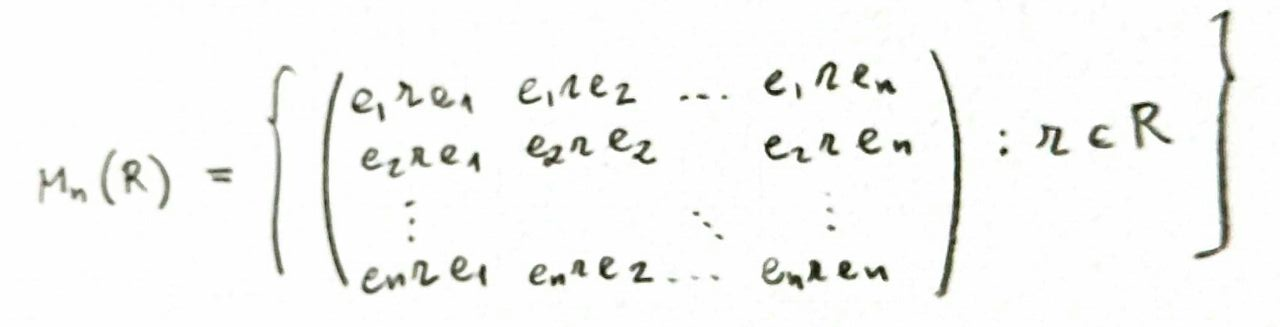
\includegraphics[width=10cm]{images/mring.jpg}
\end{figure}

is also idempotented ring and that every idempotented ring is isomorphic to a matrix ring.
\end{example}

\begin{exercise}[Proposed to the reader]
Prove that $(R,I) \cong (M_n(R),I_{M_n(R)})$. 

Hint: you may use $\phi(r) = (e_jre_i)$ as isomorphism.
\end{exercise}


\textbf{Category of idempotented rings}

The category of idempotented rings, Ring$_\perp$ is given by $Ob(Ring_\perp) = $ idempotented rings and $Mor_{Ring_\perp}((R, I),(S, J)) = $ homomorphisms $h: R \to S$ such that $h(e) \in J$ for all $e \in I$.

Note that this last condition is unnecessary to be mentionned since any ring homomorphism preserves idempotents as: $$e \in I \implies e^2 = e \implies h(e) = h(e)^2 \implies h(e) \in J$$


\end{definition}

\subsection{Definitions in category theory}

\begin{definition}[Notions on categories]

\textbf{Small category}

A category C is small if the class of objects and the class of morphisms are both sets.

\textbf{Preadditive category}

A category $C$ is preadditive if for any $X,Y \in Ob(C)$, $Mor_C(X,Y)$ has the structure of an abelian group, which we write additively. Furthermore, we require that composition is distributive over this addition.

\textbf{Additive functor}

Suppose C and D are preadditive categories. 

A functor $F : C \to D$ is additive if for all $X, Y \in Ob(C), F : Mor_C(X, Y ) \to Mor_D(F (X), F (Y ))$ is a group homomorphism with respect to addition.

\textbf{Category of small preadditive categories with one object}

Let PreCat$_1$ denote the category of small preadditive categories with one object. The objects are small preadditive categories with one object and $Mor_{PreCat_1}(C, D)$ is the class of additive functors from C to D.

\textbf{Category of small preadditive categories with finitely many objects}

Let PreCat$_{Fin}$ denote the category of small preadditive categories with finitely many objects. The objects are small preadditive categories with finitely many objects and MorPreCat$_{Fin}(C, D)$ is the class of additive functors from $C$ to $D$.

\textbf{Split idempotent}

A morphism $e \in Mor_C(X,X)$ is idempotent if $e \circ e = e$.

An idempotent $e$ is an split idempotent if $\exists f \in Mor_C(X,Y), g \in Mor_C(Y,X).g \circ f = e \land f \circ g = id_Y$.


\begin{figure}[H]
\centering
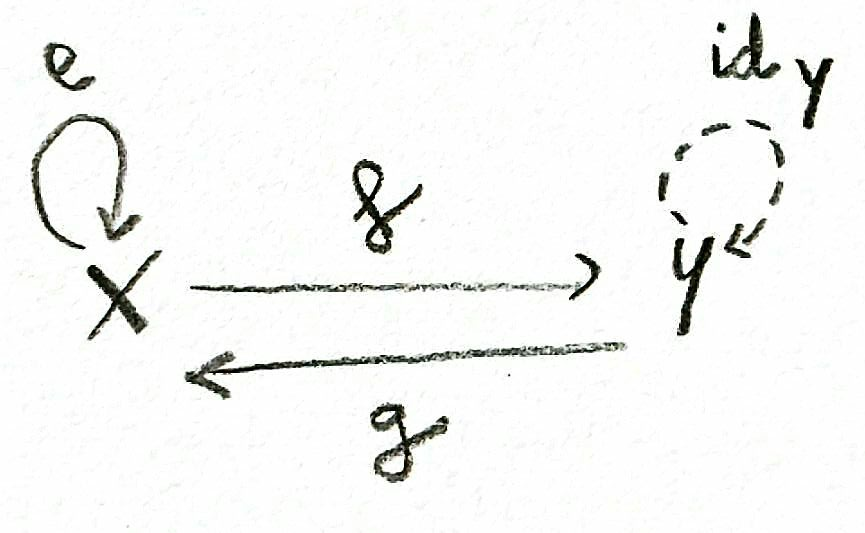
\includegraphics[width=4cm]{images/idempotent.jpg}
\end{figure}

\textbf{Idempotent complete category}

A category $C$ is idempotent complete if every idempotent morphism in $C$ is a split idempotent.
\end{definition}

\begin{definition}[Notions on relations between categories]
Suppose $C$ and $D$ are categories and $F, G: C \to D$ functors. A natural transformation $\eta$ from $F$ to $G$, denoted as $\eta : F \to G$, is a mapping from $Ob(C)$ to $Mor(D)$ that associates every $X \in Ob(C)$ to a morphism $\eta_X \in Mor_D(F(X), G(X))$ such that the following diagram commutes for any $f \in Mor_C(X, Y )$.

\begin{figure}[H]
\centering
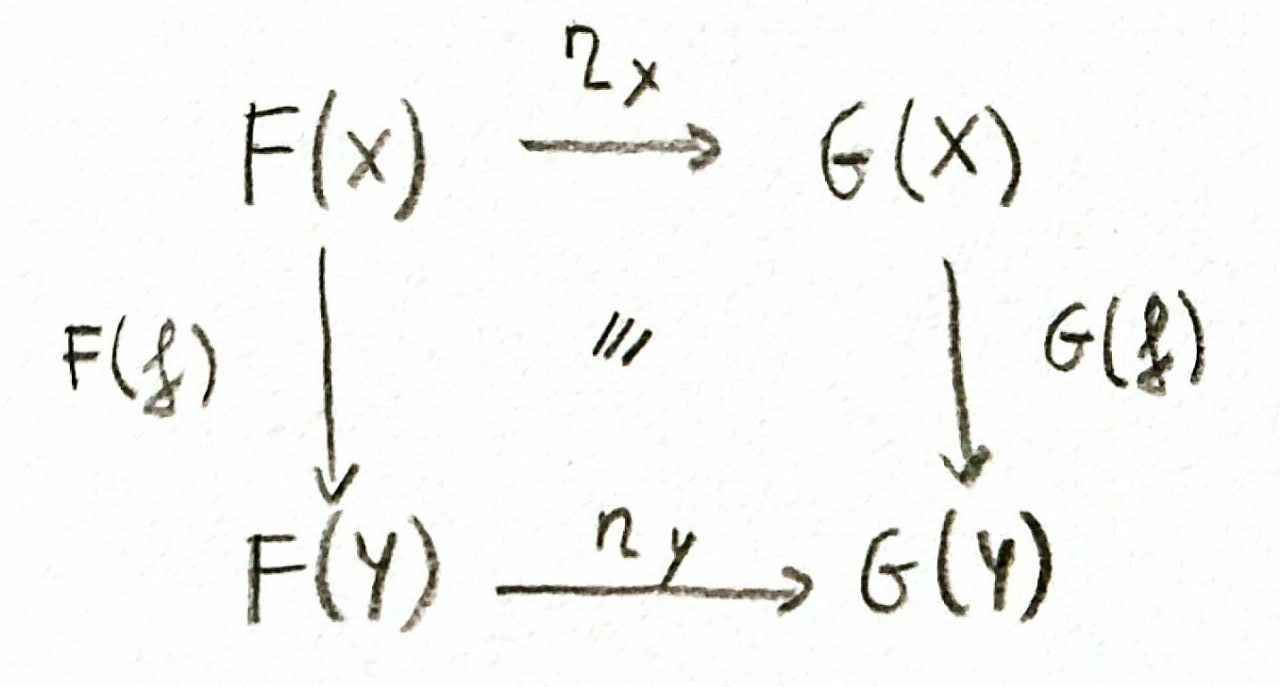
\includegraphics[width=4cm]{images/natural.jpg}
\end{figure}

If $\eta_X:F(X) \to G(X)$ is an isomorphism (there exists an inverse functor) for all $X \in Ob(C)$, then $\eta$ is a natural isomorphism.



\textbf{Equivalence of categories}

Two categories $C$ and $D$ are equivalent (written as $C \simeq D$) if there exists a pair of functors $F : C \to D$, $G: D \to C$ and a pair of natural isomorphisms $\eta: id_C \to G \circ F$, $\epsilon: id_D \to F \circ G$.

Let $C$ and $D$ be categories. Recall that a functor $F : C \to D$ gives rise to map $F_{X,Y} : Mor_C(X,Y) \to Mor_D(F (X), F (Y ))$, for all $X, Y \in Ob(C)$. 

\textbf{Full functor}

The functor $F$ is full on morphisms if $F_{X,Y}$ is surjective for all $X, Y \in Ob(C)$.

\textbf{Faithful functor}

The functor $F$ is faithful on morphisms if $F_{X,Y}$ is injective for all $X, Y \in Ob(C)$. 

\textbf{Fully faithful functor}

If $F$ is both full and faithful, it is called fully faithful.

\textbf{Essentially surjective}

Suppose $C$ and $D$ are categories. A functor $F : C \to D$ is essentially surjective on objects if for all $Y \in Ob(D)$, there exists a $X \in Ob(C)$ such that $F(X) \cong Y $ (objects are isomorphic).

\end{definition}

Equivalences are good because they preserve many (but not every categorical property). Intuitively, one is saying that up to a natural transformation $F,G$ are one the inverse of the other. 

The following result allows to check a list of properties that depend on one morphism instead of proving explicitly the natural transformations.

\begin{theorem}[Maclane]
Suppose $C$ and $D$ are categories and $F : C \to D$ a functor. The functor $F$ yields an equivalence of categories if and only if $F$ is fully faithful on morphisms and essentially surjective on objects.
\end{theorem}




